% =====================================================================
%  PHỤ LỤC F. BẢN SAO THUYẾT MINH VÀ HỢP ĐỒNG
%  (Phụ lục hướng dẫn, mục 3.14: đóng kèm 1 bản sao Thuyết minh và Hợp đồng
%   đã được phê duyệt vào cuối cuốn báo cáo tổng kết.)
%  Scan hợp đồng đã ký rồi lưu thành tailieu_goc/hop_dong.pdf, biên dịch lại
%  là tự động đóng vào sau thuyết minh. Nếu chưa có tệp, phần này tự bỏ qua
%  và bạn kẹp bản scan/bản photo vào cuối cuốn khi đóng quyển.
% =====================================================================
\chapter{Bản sao thuyết minh và hợp đồng đã được phê duyệt}
\label{pl:f}
Phụ lục này gồm bản sao thuyết minh đề tài nghiên cứu khoa học sinh viên năm 2026 (mẫu BM02/QT-PKHCN-NCKHSV/00, mã số \madetai) và bản sao hợp đồng thực hiện đề tài đã được phê duyệt.
\clearpage
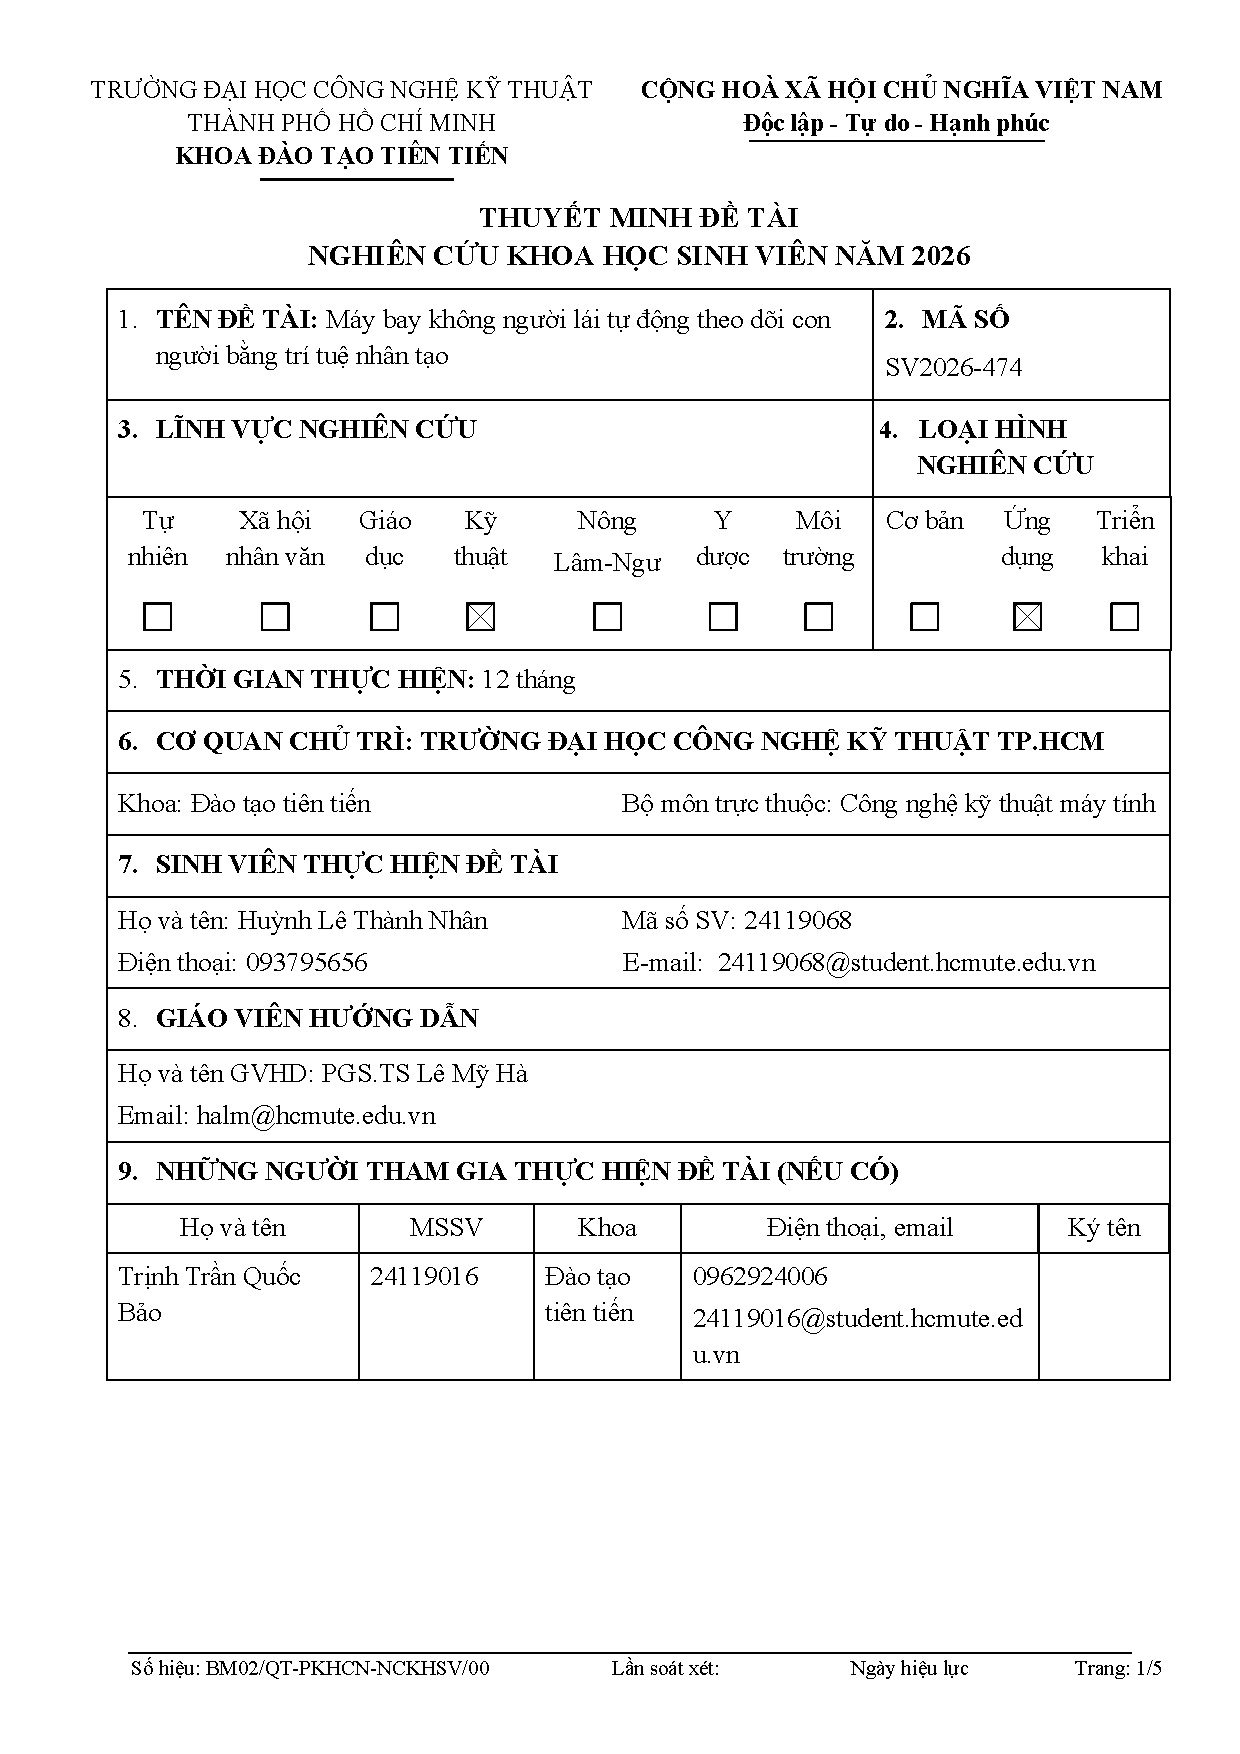
\includepdf[pages=-,scale=0.92,pagecommand={\thispagestyle{plain}}]{../tailieu_goc/BM02_NCKH_HuynhLeThanhNhan_v3.pdf}
\IfFileExists{../tailieu_goc/hop_dong.pdf}{%
  \includepdf[pages=-,scale=0.92,pagecommand={\thispagestyle{plain}}]{../tailieu_goc/hop_dong.pdf}}{}
